% Created 2021-10-13 Wed 17:50
% Intended LaTeX compiler: pdflatex
\documentclass[presentation,aspectratio=169]{beamer}
\usepackage[utf8]{inputenc}
\usepackage[T1]{fontenc}
\usepackage{graphicx}
\usepackage{grffile}
\usepackage{longtable}
\usepackage{wrapfig}
\usepackage{rotating}
\usepackage[normalem]{ulem}
\usepackage{amsmath}
\usepackage{textcomp}
\usepackage{amssymb}
\usepackage{capt-of}
\usepackage{hyperref}
\usepackage{pifont}
\newcommand{\cmark}{\textcolor{green!80!black}{\ding{51}}}
\usepackage{amssymb}
\usepackage{pgfplotstable}
\DeclareMathOperator{\shift}{q}
\DeclareMathOperator{\diff}{p}
\usepackage{khpreamble, euscript, mathtools}
\DeclareMathOperator{\atantwo}{atan2}
\newcommand*{\ctrb}{\EuScript{C}}
\newcommand*{\obsv}{\EuScript{O}}
\usetheme{default}
\author{Kjartan Halvorsen}
\date{\today}
\title{State feedback with observer}
\hypersetup{
 pdfauthor={Kjartan Halvorsen},
 pdftitle={State feedback with observer},
 pdfkeywords={},
 pdfsubject={},
 pdfcreator={Emacs 26.3 (Org mode 9.4.6)}, 
 pdflang={English}}
\begin{document}

\maketitle



\section{State feedback with observer}
\label{sec:org6a704fe}
\begin{frame}[label={sec:org7a0da2a}]{State feedback with reconstructed states}
\end{frame}

\begin{frame}[label={sec:orge158726}]{State feedback with reconstructed states}
\begin{center}
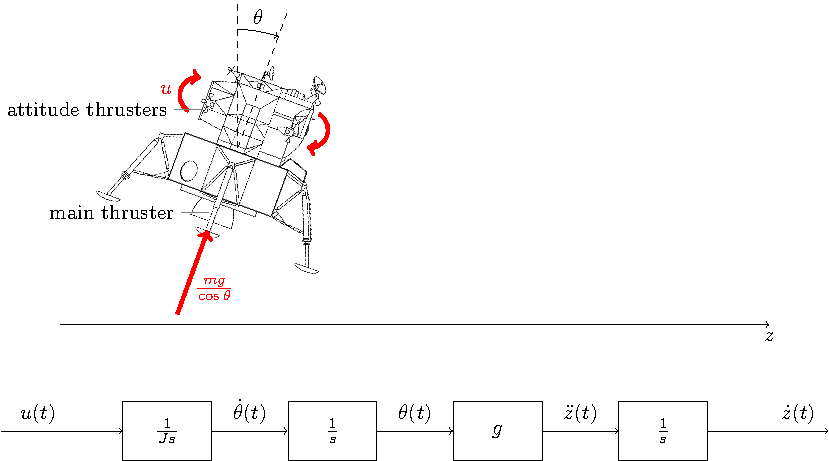
\includegraphics[width=0.9\linewidth]{../../figures/fig-apollo}
\end{center}
\end{frame}

\begin{frame}[label={sec:orgba6ddde}]{State feedback}
Given
 \begin{equation}
 \begin{split}
  \dot{x} &= A x + B u\\
  y &= C x
 \end{split}
 \label{eq:ssmodel}
\end{equation}
and measurements (or estimates) of the state vector \(x\). 

\alert{Linear state feedback} is the control law
\begin{equation*}
\begin{split}
 u &= f\big((x, u_c\big) = -l_1x_1 - l_2x_2 - \cdots - l_n x_n + l_0u_c\\
      &= -\textcolor{morange}{L}x + l_0u_c, 
\end{split}
\end{equation*}
where \[ \textcolor{morange}{L} = \bbm l_1 & l_2 & \cdots & l_n \ebm. \]
Substituting the control law in the state space model \eqref{eq:ssmodel} gives
 \begin{equation}
 \begin{split}
  \dot{x} &= \left(A -B \textcolor{morange}{L} \right) x + l_0B r\\
  y(k) &= C x
 \end{split}
 \label{eq:closedloop}
\end{equation}
\end{frame}



\begin{frame}[label={sec:orgd40e8ca}]{Observer design}
Given model
 \begin{equation*}
 \begin{split}
  \dot{x} &= A x + B u\\
  y &= C x
 \end{split}
 \label{eq:ssmodel}
\end{equation*}
and measurements of the output signal \(y\). 

The observer is given by
\begin{equation*}
\begin{split}
\dot{\hat{x}} &= \underbrace{A \hat{x} + B u{}}_{\text{simulation}} + \underbrace{\textcolor{mred}{K}\big(y - C\hat{x}\big)}_{\text{correction}} = \left(A - \textcolor{mred}{K}C\right)\hat{x} +  B u{} + \textcolor{mred}{K}y
\end{split}
\end{equation*}
with poles given by the eigenvalues of the matrix \(A_o = A - \textcolor{mred}{K}C\)

\alert{Rule-of-thumb} Choose the poles of the observer (eigenvalues of \(A-\textcolor{mred}{K}C\)) at least twice as fast as the poles (eigenvalues) of \(A-B \textcolor{morange}{L}\).
\end{frame}

\begin{frame}[label={sec:orgf937913}]{Observer design}
\alert{Rule-of-thumb} Choose the poles of the observer (eigenvalues of \(A-\textcolor{vmermillion}{K}C\)) at least twice as fast as the poles (eigenvalues) of \(A-B \textcolor{morange}{L}\).
\end{frame}


\begin{frame}[label={sec:org54e87b4}]{Control by feedback from reconstructed states}
The design problem can be separates into two problems
\begin{enumerate}
\item Determine the gain vector \(\textcolor{orange!80!black}{L}\) and the gain \(l_0\) of the control law
\[ u{} = -\textcolor{orange!80!black}{L} \hat{x} + l_0 r\]
so that the closed-loop system has good reference tracking.
\item Determine the gain vector \(\textcolor{mred}{K}\) of the observer
\begin{equation*}
\begin{split}
\dot{\hat{x}} &= A \hat{x} + B u{} + \textcolor{mred}{K} \big(y - C\hat{x}\big)
\end{split}
\end{equation*}
to get a good balance between disturbance rejection and noise attenuation.
\end{enumerate}
\end{frame}

\begin{frame}[label={sec:org9c64285}]{Computing the observer gain}
A matrix \(M\) and its transpose \(M\transp\) have the same eigenvalues. Hence, the problem of determining the gain \(K\) to obtain desired eigenvalues of 
\[A- \textcolor{mred}{K}C\] is equivalent to determining the gain \(\textcolor{mred}{K}\) in 
\[(A-\textcolor{mred}{K}C)\transp = A\transp - C\transp \textcolor{mred}{K}\transp.\]
The last problem has the exact same form as the problem of determining \(\textcolor{morange}{L}\) to obtain desired eigenvalues of 
\[A - B \textcolor{morange}{L}\]

So, the same matlab function can be used for both problems.
\end{frame}

\begin{frame}[label={sec:org4bcad0e},fragile]{Computing the observer gain}
 \begin{enumerate}
\item \alert{Ackerman's method} 
\begin{verbatim}
K = acker(Phi', C', po)'
\end{verbatim}
\item \alert{More numerically stable method} 
\begin{verbatim}
K = place(Phi', C', pd)'
\end{verbatim}
\end{enumerate}
\end{frame}
\end{document}